\section{Balance of the signed mass}
\label{sec:balance}

Read the height $z_c$ of a cell as a \emph{signed mass} sitting at the planar position $(x_c,y_c)$, or as the vertical coordinate of the point $(x_c,y_c,z_c)$.
A weighted configuration is \emph{balanced} for an assignment of vectors $u_c$ to the cells if the vector sum $B=\sum_cz_c\,u_c$ vanishes.
The orthogonality formulation decides which assignments are balanced by every magic square (those whose components lie in the line space, \Cref{thm:linear_balance}), gives a quantitative version for near-magic arrangements (\Cref{thm:quant_balance}), and shows that the natural nonlinear assignments by unit vectors are not (\Cref{prop:unit_negative}).
\Cref{tab:readings} summarises three physical readings and which balance conditions each yields.

\begin{table}[htbp]
\centering
\small
\renewcommand{\arraystretch}{1.25}
\begin{tabular}{>{\raggedright\arraybackslash}p{3.0cm} >{\raggedright\arraybackslash}p{3.2cm} >{\raggedright\arraybackslash}p{4.5cm} >{\raggedright\arraybackslash}p{4.0cm}}
\toprule
reading & configuration & implied by $\Efull=0$ & not implied \\
\midrule
\textbf{flat plate} (Loly): mass $s_c$ at $(x_c,y_c)$ & planar masses, centred grid & total mass $\sum s_c$ (fixed); centre of mass at the origin; axial moments $\sum s_cx_c^k$, $\sum s_cy_c^k$; moment of inertia $I=\sum s_c(x_c^2+y_c^2)=\frac{n^2(n^4-1)}{12}$ (semi-magic suffices) & mixed moments, e.g.\ the product of inertia $\sum s_cx_cy_c$ (\Cref{thm:linear_balance}(d)) \\
\textbf{ring / top}: weight $z_c$ at angle $\theta_c$ of cell $c$ & points on the unit circle, $u_c=(\cos\theta_c,\sin\theta_c)$ & only the total weight $\sum z_c=0$ & $B_{\mathrm{ring}}=0$ ($B_{\mathrm{ring}}=2.62$ for all eight $3\times3$ magic squares) \\
\textbf{vectors from the centroid}, signed mass $z_c$ & $v_c=(x_c,y_c,z_c)$; linear sums $\sum z_cv_c$ and unit-vector sums $\sum z_cv_c/|v_c|$ & linear: horizontal part $\sum z_c(x_c,y_c)=0$ and all separable moments; the vertical part $\sum z_c^2=N\Var Z$ is fixed and positive & unit-vector sum: horizontal part (\Cref{prop:unit_negative}(a)); the vertical part $V>0$ for every arrangement \\
\bottomrule
\end{tabular}
\caption{Three readings of a magic square as a weighted configuration, and the balance conditions that follow from $\Efull=0$. The plate reading uses the planar masses $s_c$; the other two use the signed heights $z_c$.}
\label{tab:readings}
\end{table}


Let $\mathcal L=\R\mathbf 1\oplus W$ denote the span of the constant function and the $2n+2$ line indicators (\Cref{lem:W_structure}); $\dim\mathcal L=2n+1$.
Recall $\langle f,g\rangle=\frac1N\sum_cf_cg_c$, so that $\sum_cz_c\varphi_c=N\langle z,\varphi\rangle$.

\subsection{Linear balance}
\label{sec:balance_linear}

\begin{theorem}[Linear balance]
\label{thm:linear_balance}
Let $S$ be an arrangement of order $n\ge3$ with height function $z$.
\begin{enumerate}
\item[(a)] $\Efull(S)=0$ if and only if $\sum_cz_c\varphi_c=0$ for every $\varphi\in\mathcal L$.
\item[(b)] If $S$ is magic, then for all functions $a,b:\{0,\dots,n-1\}\to\R$ and all $c_1,c_2\in\R$,
\begin{equation}
\sum_{i,j}z_{ij}\Bigl(a(x_{ij})+b(y_{ij})+c_1\mathbf 1_{D_{\mathrm m}}(i,j)+c_2\mathbf 1_{D_{\mathrm a}}(i,j)\Bigr)=0 .
\label{eq:linear_balance}
\end{equation}
In particular $\sum_cz_c=0$ (true for every arrangement), the centre of mass vanishes, $\sum_cz_c(x_c,y_c)=0$, every axial moment vanishes, $\sum_cz_cx_c^{k}=\sum_cz_cy_c^{k}=0$ for all $k\ge0$, and Loly's invariant holds, $\sum_cz_c(x_c^2+y_c^2)=0$ (\Cref{cor:loly}).
For the physical mass $s_c=z_c+\frac{N+1}2$ the centre of mass is the origin and every axial moment equals that of a uniform plate of the same total mass.
\item[(c)] For (b) with $c_1=c_2=0$ it suffices that $S$ is semi-magic.
\item[(d)] The mixed moments are not determined: for the magic square
\[
\begin{pmatrix}1&6&11&16\\8&15&2&9\\12&3&14&5\\13&10&7&4\end{pmatrix}
\]
one has $\sum_cz_cx_cy_c=60$, and $\sum_cz_cx_cy_c\ne0$ for $824$ of the $880$ essentially different magic squares of order~$4$ (the same holds for $\sum_cz_cx_c^2y_c$ and $\sum_cz_cx_cy_c^2$ for $623$ and $773$ of them).
For $n=3$ it vanishes for all eight magic squares.
\end{enumerate}
\end{theorem}

\begin{proof}
(a) $\mathbf 1^{\perp}\ni z$ for every arrangement (\Cref{lem:variances}), so $z\perp\mathcal L$ if and only if $z\perp W$, which by \Cref{lem:zero_set} is equivalent to $\Efull(S)=0$.
(b) $a(x)=\sum_\ell a(x_\ell)C_\ell$ lies in the span of the column indicators, $b(y)$ in that of the row indicators, and the diagonal indicators lie in $W+\R\mathbf 1$; apply (a).
The special cases are $a=1$; $a(x)=x^k$, $b(y)=y^k$; and $a(x)=x^2$, $b(y)=y^2$.
For the statement about $s$: $\sum_cs_c(x_c,y_c)=\sum_cz_c(x_c,y_c)+\frac{N+1}2\sum_c(x_c,y_c)=0$, and $\sum_cs_cx_c^k=\frac{N+1}2\sum_cx_c^k$.
(c) is \Cref{prop:hierarchy}(a).
(d) The displayed square has all line sums $34$; the counts for $880$ squares are computed by enumeration.
For $n=3$ every magic square has $s_c+s_{c'}=10$ for centrally opposite cells $c,c'$, so $z$ is odd under $(x,y)\mapsto(-x,-y)$ while $xy$ is even.
\end{proof}

The linear moments of low degree therefore carry no information beyond $\Efull=0$, and one cannot hope for more from line sums alone: since $xy\notin\mathcal L$ (part (d) exhibits magic squares with $\sum_cz_cx_cy_c\ne0$), the mixed moments vary over magic squares.

\begin{theorem}[Quantitative linear balance]
\label{thm:quant_balance}
Let $S$ be any arrangement of order $n\ge3$ and let $E_{\mathrm{rc}}=\sum_k\Cov(R_k,Z)^2+\sum_\ell\Cov(C_\ell,Z)^2\ (\le\Efull)$ be the energy of the rows and columns.
\begin{enumerate}
\item[(a)] $\displaystyle \Cov(X,Z)^2+\Cov(Y,Z)^2\ \le\ \frac{n(n^2-1)}{12}\,E_{\mathrm{rc}}$, equivalently
\begin{equation}
\Bigl|\sum_cz_c(x_c,y_c)\Bigr|^2\ \le\ N^2\,\frac{n(n^2-1)}{12}\,E_{\mathrm{rc}}\ \le\ N^2\,\frac{n(n^2-1)}{12}\,\Efull .
\label{eq:T2}
\end{equation}
\item[(b)] The constant $n(n^2-1)/12$ cannot be improved, for any $n$: equality holds for the natural arrangement $s_{ij}=in+j+1$ (and, more generally, for every real height function $z=\alpha x+\beta y$), with equality throughout \eqref{eq:T2}.
\item[(c)] For every $\varphi\in W$, $\ \bigl|\sum_cz_c\varphi_c\bigr|\le N\,\|\varphi\|\,\dfrac{n}{\sqrt{n-2}}\sqrt{\Efull}$, where $\|\varphi\|^2=\frac1N\sum_c\varphi_c^2$.
\end{enumerate}
\end{theorem}

\begin{proof}
(a) With $\gamma_\ell=\sum_iz_{i\ell}$ the column sums and $\rho_k$ the row sums, $\sum_cz_cx_c=\sum_\ell x_\ell\gamma_\ell$ and $\sum_cz_cy_c=\sum_ky_k\rho_k$, where $\sum_\ell x_\ell^2=\sum_ky_k^2=n(n^2-1)/12$.
Cauchy--Schwarz gives $(\sum_cz_cx_c)^2+(\sum_cz_cy_c)^2\le\frac{n(n^2-1)}{12}(\|\gamma\|^2+\|\rho\|^2)$, and $\|\gamma\|^2+\|\rho\|^2=N^2E_{\mathrm{rc}}$ by \Cref{lem:variances}(3).
Dividing by $N^2$ gives the covariance form.
(b) For the natural arrangement $z=x-ny$ the column sums are $\gamma=nx$ and the row sums $\rho=-n^2y$, proportional to $x$ and $y$, which is the equality case of both Cauchy--Schwarz steps; both diagonal sums vanish, so $E_{\mathrm{rc}}=\Efull$.
In general equality in (a) holds iff $\gamma\parallel x$ and $\rho\parallel y$.
(c) By \Cref{lem:projection}, $\|P_{W_R}z\|^2=n\|\rho\|^2/N^2$, $\|P_{W_C}z\|^2=n\|\gamma\|^2/N^2$ and $\|P_{W_D}z\|^2=\frac1N\delta^{\mathsf T}G^{-1}\delta$ with $\delta^{\mathsf T}\delta/N^2$ the diagonal part of $\Efull$.
The eigenvalues of $G$ are $n-1$ (twice) for odd $n$ and $n-2,\,n$ for even $n$, so $\frac1N\delta^{\mathsf T}G^{-1}\delta\le\frac{N}{n-2}\,\delta^{\mathsf T}\delta/N^2$, and
$n\,\Efull\le\|P_Wz\|^2\le\max\{n,\tfrac{N}{n-2}\}\Efull=\tfrac{n^2}{n-2}\Efull$.
For $\varphi\in W$, $\sum_cz_c\varphi_c=N\langle P_Wz,\varphi\rangle\le N\|\varphi\|\|P_Wz\|$.
\end{proof}

Part (a) is a stability statement: the linear imbalance of the centre of mass is controlled by the energy, with a constant that depends only on $n$ and is attained; for $\Efull=0$ it recovers the centre-of-mass part of \Cref{thm:linear_balance}.
Numerically, inequality \eqref{eq:T2} has no violation on all $9!$ arrangements for $n=3$ (the ratio of the two sides reaches $1$, at $4152$ arrangements including the natural one), on $3\times10^5$ random arrangements for $n=4$ (maximal ratio $0.998$) and on $10^5$ random arrangements for each of $n=5,6,7$ (maximal ratios $0.977,\,0.944,\,0.903$); see \Cref{fig:balance}(a).
In (c), the observed ratio $\|P_Wz\|^2/\Efull$ over $2\times10^4$ random arrangements lies in $[n,\,7.38]$ for $n=4$, consistent with $[n,\,n^2/(n-2)]=[4,8]$.

\subsection{Nonlinear balance by unit vectors}
\label{sec:balance_unit}

Two assignments of unit vectors are natural.
In the \emph{ring} reading each cell $c\ne$ centre is projected radially onto the unit circle, $u_c=(x_c,y_c)/r_c$ with $r_c=\sqrt{x_c^2+y_c^2}$ (and $u_c=0$ at the centre cell when $n$ is odd), and carries the weight $z_c$:
\[
B_{\mathrm{ring}}(S)=\Bigl|\sum_cz_c\,u_c\Bigr| .
\]
In the \emph{three-dimensional} reading the vectors $v_c=(x_c,y_c,z_c)$ from the centroid are normalised, $u_c'=v_c/|v_c|$ (and $u_c'=0$ if $v_c=0$), and carry the weight $z_c$.
Write $B_{3\mathrm D}^{xy}$ for the horizontal part of $\sum_cz_cu_c'$ and $V(S)=\sum_cz_c^2/|v_c|$ for its vertical part.
Both are invariant under $D_4$, because $z(gS)=g\,z(S)$ and $u_{gc}=g\,u_c$.

\begin{proposition}[Unit-vector balance is not implied]
\label{prop:unit_negative}
\begin{enumerate}
\item[(a)] Each of the eight magic squares of order $3$ has $\Efull=0$ and
$B_{\mathrm{ring}}=2(2-\sqrt2)\sqrt5\approx2.6197>0$ and $B^{xy}_{3\mathrm D}\approx1.5279>0$.
\item[(b)] For every arrangement of every order, $V(S)\ge\sum_cz_c^2/\max_c|v_c|>0$; consequently the three-dimensional vector sum $\sum_cz_cu_c'$ is nonzero for \emph{every} arrangement, magic or not.
\item[(c)] If $u_c=(F(x_c),G(y_c))$ with functions $F,G$ of one coordinate each (for example the linearisation $u_c=(x_c,y_c)/r_0$ with a constant $r_0$), then $\Efull(S)=0$ implies $\sum_cz_cu_c=0$ (\Cref{thm:linear_balance}); the radial unit vectors do not have this form.
\end{enumerate}
\end{proposition}

\begin{proof}
(a) By $D_4$-invariance it suffices to take the Lo~Shu square with rows $(2,7,6),(9,5,1),(4,3,8)$, so $z=s-5$.
The four edge cells have $u=(\pm1,0),(0,\pm1)$ and heights $z=-4$ (right), $4$ (left), $2$ (top), $-2$ (bottom), contributing $(-8,4)$; the four corners have $u=(\pm1,\pm1)/\sqrt2$ and heights $-3,1,-1,3$ (upper left, upper right, lower left, lower right), contributing $(8,-4)/\sqrt2=(4\sqrt2,-2\sqrt2)$.
The total is $(4\sqrt2-8,\,4-2\sqrt2)=(4-2\sqrt2)(-2,1)$, of norm $(4-2\sqrt2)\sqrt5$.
The value of $B^{xy}_{3\mathrm D}$ is obtained in the same way, numerically.
(b) $V=\sum_cz_c\cdot z_c/|v_c|$ and $z_c\ne0$ for all but at most one cell.
(c) is \Cref{thm:linear_balance}(b).
\end{proof}

\begin{remark}[Reading of \Cref{prop:unit_negative}]
\label{rem:unit_reading}
The negative statement is about implication only.
Statement~(a) shows that $\Efull=0$ does not imply the vanishing of the ring imbalance, and (b) shows that the vanishing of a full three-dimensional unit-vector sum is impossible for \emph{any} arrangement, because the vertical component is a sum of squares.
The comparison below shows, however, that magic squares are not typical in the unit-vector imbalance either.
\end{remark}

\paragraph{Numerical comparison, $n=4$.}
\Cref{tab:unit_n4} compares the $880$ essentially different magic squares of order~$4$ with $3\times10^5$ uniformly random arrangements (fixed seed, \texttt{anc/balance\_check.py}).
The linear imbalance vanishes on every magic square, as it must (\Cref{thm:linear_balance}), and is nonzero for $99.97\%$ of random arrangements.
The unit-vector imbalances of magic squares are smaller than those of random arrangements on average, the mean over magic squares lying below the $7.4\%$ (ring) and $2.4\%$ (three-dimensional, horizontal) quantiles of the random distribution; but they never vanish (smallest values $0.070$ and $0.036$), and the largest magic value of $B_{\mathrm{ring}}$ is the $31$st percentile of the random distribution (\Cref{fig:balance}(b,c)).
Among random arrangements the Spearman correlation between $\Efull$ and $B_{\mathrm{lin}}$, $B_{\mathrm{ring}}$, $B_{3\mathrm D}^{xy}$ is $0.38$, $0.33$, $0.34$.
The vertical component $V$ of the three-dimensional model is $59.57$ on average for magic and for random arrangements alike: it is close to $\sum_c|z_c|=64$, a constant, because $|v_c|\approx|z_c|$ for most cells, and carries no information about the line sums.
For $n=3$, over all $9!$ arrangements the smallest value of $B_{\mathrm{ring}}$ is $0.131$, and $9.1\%$ of the arrangements have a smaller ring imbalance than the magic squares ($2.62$).

\begin{table}[htbp]
\centering
\small
\begin{tabular}{l rrr rr}
\toprule
 & \multicolumn{3}{c}{880 magic squares ($n=4$)} & \multicolumn{2}{c}{$3\times10^5$ random} \\
\cmidrule(lr){2-4}\cmidrule(lr){5-6}
imbalance & mean & min & max & mean & rank of magic mean \\
\midrule
$B_{\mathrm{lin}}=|\sum_cz_c(x_c,y_c)|$ & $0$ & $0$ & $0$ & $27.03$ & $0.03\%$ \\
$B_{\mathrm{ring}}$ & $5.51$ & $0.070$ & $11.98$ & $17.06$ & $7.4\%$ \\
$B^{xy}_{3\mathrm D}$ & $0.874$ & $0.036$ & $2.54$ & $4.90$ & $2.4\%$ \\
$|\sum_cz_cx_cy_c|$ & $19.9$ & $0$ & $60$ & $19.3$ & $57\%$ \\
\bottomrule
\end{tabular}
\caption{Balance functionals on the $880$ essentially different magic squares of order $4$ and on $3\times10^5$ uniformly random arrangements. ``Rank'' is the percentage of random arrangements with a smaller value than the mean over the magic squares. The mixed moment $|\sum_cz_cx_cy_c|$ is not controlled by $\Efull$ and is indistinguishable between the two groups.}
\label{tab:unit_n4}
\end{table}

\begin{figure}[htbp]
\centering
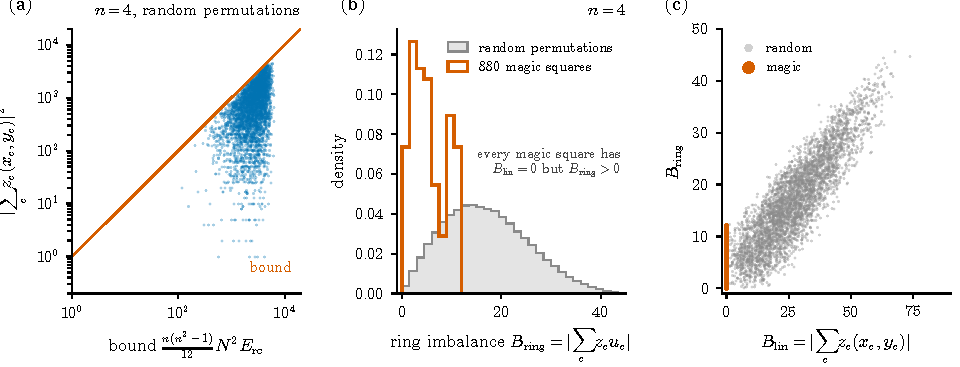
\includegraphics[width=\textwidth]{figures/fig_balance.pdf}
\caption{Balance of the signed mass for $n=4$. (a) The bound \eqref{eq:T2}: the squared linear imbalance $|\sum_cz_c(x_c,y_c)|^2$ against $\frac{n(n^2-1)}{12}N^2E_{\mathrm{rc}}$ for $4000$ random arrangements; the line is the bound, which is attained. (b) Distribution of the ring imbalance $B_{\mathrm{ring}}=|\sum_cz_cu_c|$ for $3\times10^5$ random arrangements (grey) and for the $880$ magic squares (orange outline): magic squares are smaller than typical but never zero. (c) Linear against ring imbalance: every magic square lies on the axis $B_{\mathrm{lin}}=0$ at a positive value of $B_{\mathrm{ring}}$.}
\label{fig:balance}
\end{figure}

\begin{remark}[A relaxed gradient flow]
\label{rem:flow}
Let $z$ be a real-valued height function and consider the gradient flow $\dot z=-\nabla\Efull(z)$ of the quadratic form \eqref{eq:Efull}.
It is linear, and its limit is the orthogonal projection of the initial height onto the zero set $W^{\perp}$, i.e.\ $z_\infty=z_0-P_Wz_0$.
By \Cref{thm:linear_balance} the limit has $\Efull=0$ and exactly zero linear imbalance.
It does not balance the ring: starting from uniformly random permutations for $n=4$ ($2\times10^4$ starts), the mean of $B_{\mathrm{ring}}$ decreases from $17.1$ to $3.9$ (and that of $B_{3\mathrm D}^{xy}$ from $4.9$ to $1.5$), so the limit is balanced linearly but not on the ring.
\end{remark}

\subsection{Multipole moments}
\label{sec:balance_multipole}

\begin{remark}[Multipole moments]
\label{rem:multipole}
The sums $m_{ab}=\sum_cz_cx_c^ay_c^b$ are the Cartesian moments of the signed planar distribution $z$; the monopole is $m_{00}$, the dipole $(m_{10},m_{01})$, and the quadrupole is built from $m_{20},m_{02},m_{11}$.
Rogers and Loly studied the electric multipole expansion of a magic cube regarded as a charge distribution \cite{rogers2005multipole}.
In the present notation, \Cref{thm:linear_balance} says that for a magic square every \emph{pure} moment $m_{a0}$, $m_{0b}$ vanishes, so the monopole, the dipole and the diagonal quadrupole components $m_{20},m_{02}$ (hence the trace and the traceless part $m_{20}-m_{02}$) vanish, whereas the mixed moments $m_{ab}$ with $a,b\ge1$, beginning with $m_{11}$, are not determined by the line sums.
The hierarchy of \Cref{prop:hierarchy} is the statement that, for real height functions, the vanishing of the pure axial moments up to degree $n-1$ in each coordinate is \emph{equivalent} to equal row and column sums, and that fewer moments do not suffice.
We make no claim beyond this algebraic correspondence.
\end{remark}
